%================================================================
\chapter{Interferometry}
\chaptermark{Chapter 3}
%================================================================





%==============================
\section{Introduction}

Atomic interferometry involves coherently manipulating the translational motion of atoms in order to obtain extremely precise information about a physical system. The idea extends principles more
familiar in optical interferomtery to atoms. The wave nature of atoms and molecules allows us to interfere these particles with each other in order to extract information about the imposed system. In particular, atom interferometry offers a unique window from which to view the Aharonov-Bohm, Aharonov-Cacher, and He-McKellar-Wilkens effects.  These topological effects are only accessible to experiments which are able to interfere atoms - revealing the phase nature of atoms, hidden from classical experiments.  In this section we will review the path integral formulation of classical mechanics which will lead us to a simple way to calculate the quantum phase picked up by atoms due to various perturbations. With the necessary mathematical tools under our belt, we introduce the Mach-Zehnder inteferometer and apply a traveling wave perturbation along each ineterferometer arm in order to induce an HMW phase.  We show that under a carefully setup experiment, it is possible, for the first time, to observe the optical He-McKellar-Wilkens phase.  Two other setups are then introduced: the Kapitza-Dirac interferometer, and the Laguerre beam interferometer.  These experiments offer alternative opportunities to probe the faint topological phase.

%_________________________________
\newpage

\section{Path Integrals}
In this section we introduce Feynman's approach to path integrals.  We begin with a classical treatment of the problem, and then move to a quantum interferometric system.

\subsection{Classical Mechanics}

Consider the path between two points $(\mathbf{x}_a,t_a)$ and $(\mathbf{x}_b,t_b)$.  There are infinitely many paths ${\Gamma_1, \Gamma_2,...}$ linking these two points, but only one $\Gamma_{\mathrm{cl}}$ is actually taken by the particle.  This path is determined from the classical Lagrangian of the system
\begin{equation}
L(\mathbf{x},\dot{\mathbf{x}})=\frac{1}{2}m\dot{x}^2-V(\mathbf{x})
\end{equation}
through the principle of least action (PLA).  The PLA states that $\Gamma_{\mathrm{cl}}$ is the path which extremizes the classical action
\begin{equation}
S(\Gamma_{\mathrm{cl}})=\int^{t_b}_{t_a}L(\mathbf{x}(t),\dot{\mathbf{x}}(t))\,dt
\end{equation}
To find the condition on $L$ which extremizes the action $S$ we consider a variation $\epsilon\eta(t)$ 
in the classical path. The action is then written as
\begin{equation}
S(\Gamma)=\int^{t_b}_{t_a}L(\mathbf{x}(t)+\epsilon\mathbf{\eta}(t),\dot{\mathbf{x}(t)}+\epsilon\dot{\mathbf{\eta}}(t))\,dt
\end{equation}
If we require this to be extremal with respect to $\epsilon$, then we must solve for
\begin{equation}
\frac{d}{d\epsilon}\int^{t_b}_{t_a}L(\mathbf{x}(t)+\epsilon\mathbf{\eta}(t),\dot{\mathbf{x}(t)}+\epsilon\dot{\mathbf{\eta}}(t))\,dt=0
\end{equation}
This implies that
\begin{equation}
\int^{t_b}_{t_a}\left(\frac{\partial L}{\partial x}\eta(t)-\frac{\partial L}{\partial \dot{x}}\dot{\eta}(t)\right)\,dt
\end{equation}
This may be rewritten by making use of integration by parts on the second term 
\begin{equation}
\int^{t_b}_{t_a}\frac{\partial L}{\partial \dot{x}}\dot{\eta}(t)\,dt=\left[\frac{\partial L}{\partial \dot{x}}\eta(t)\right]^{t_b}_{t_a}-\int^{t_b}_{t_a}\frac{d}{dt}\frac{\partial L}{\partial \dot{x}}\eta(t)\,dt
\end{equation} 
The first term on the right side is zero since we require the variation $\eta(t)$ to be zero at the boundary. This then leads to
\begin{equation}
\int^{t_b}_{t_a}\left[\frac{\partial L}{\partial x}\eta(t)-\frac{d}{dt}\frac{\partial L}{\partial \dot{x}}\eta(t)\right]\,dt=0
\end{equation}
which we recognize as the Euler-Lagrange equation
\begin{equation}
\frac{\partial L}{\partial x}-\frac{d}{dt}\frac{\partial L}{\partial \dot{x}}=0
\end{equation}

\vspace{5mm}

The Hamiltonian is defined as 
\begin{equation}
H=\mathbf{p}\dot{\mathbf{x}}-L
\end{equation}
where the canonical momentum $\mathbf{p}$ is given by 
\begin{equation}
\mathbf{p}=\frac{\partial L}{\partial \dot{x}}
\end{equation}
If we change the end point $(\mathbf{x}_b,t_b)$, the action varies as
\begin{equation}
dS_{\mathrm{cl}}=\frac{\partial S_{\mathrm{cl}}}{\partial x}dx+\frac{\partial S_{\mathrm{cl}}}{\partial t}dt=\mathbf{p}\,dx-H\,dt
\end{equation}
Therefore we may also write the classical action as
\begin{equation}
S_{\mathrm{cl}}=\int^{t_b}_{t_a}\left(\mathbf{p}\,dx-H\,dt\right)\,dt
\end{equation}


\subsection{The Quantum Propagator}

The final state $\ket{\psi(t_b)}$ of a quantum system is determined through an evolution operator $U$ acting on the initial state $\ket{\psi(t_a)}$
\begin{equation}
\ket{\psi(t_b)}=U\left(t_a,t_b\right)\ket{\psi(t_a)}
\end{equation}
This allows us to write the projection of the final state in the coordinate basis as
\begin{eqnarray}
\psi(\mathbf{x}_b,t_b)&=&\braket{\mathbf{x}_b|\psi(t_b)}=\braket{\mathbf{x}_b|U\left(t_a,t_b\right)|\psi(t_a)} \nonumber \\
&=&\int d\mathbf{x}_a \, \braket{\mathbf{x}_b|U\left(t_a,t_b\right)|\mathbf{x}_a}\braket{\mathbf{x}_a|\psi(t_a)} 
\end{eqnarray}

The strength of the evolution operator lies in it's ability to deal with compositions
\begin{equation}
U\left(t_a,t_c\right)=U\left(t_a,t_b\right)U\left(t_b,t_c\right)
\end{equation}
This allowed Feynman to postulate that the propagator can be thought of as a sum of contributions from all possible paths
\begin{equation}
\braket{\mathbf{x}_b|U|\mathbf{x}_a}=\mathcal{N}\sum _{\Gamma}e^{\frac{iS_{\Gamma}}{\hbar}}
\label{pathintegral1}
\end{equation}
where $\mathcal{N}$ is a normalization constant, and $\sum_{\Gamma}$ denotes the sum over all possible paths. $S_{\Gamma}/\hbar$ in Eq.\ (\ref{pathintegral1}) varies rapidly and therefore induces destructive interference - unless the path $\Gamma$ is an extremum.  In this case, constructive interference occurs between neighbouring paths.  Therefore, only paths very near to the classical path actually contribute in Eq.\ (\ref{pathintegral1}). 

\vspace{5mm}

Let us now consider quadratic Lagrangians of the form
\begin{equation}
L=a(t)\dot{x}^2+b(t)\mathbf{x}\dot{\mathbf{x}}+c(t)\dot{x}^2+d{t}\dot{\mathbf{x}}+e(t)\mathbf{x}+f(t)
\label{quadraticlagrangian}
\end{equation}
and suppose we introduce a small perturbation to the classical path $\mathbf{x}(t)=\mathbf{x}_{\mathrm{cl}}(t)+\eta(t)$.  We make sure the boundary terms still match: $\mathbf{x}_a(t)={\mathbf{x}_a}_{\mathrm{cl}}(t)$ and $\mathbf{x}_b(t)={\mathbf{x}_b}_{\mathrm{cl}}(t)$.  Then the propagator can be written as
\begin{equation}
\braket{\mathbf{x}_b|U|\mathbf{x}_a}=\int D\eta(t)\,e^{\frac{i}{\hbar}S\left[\mathbf{x}_{\mathrm{cl}}+\eta(t)\right]}
\label{pathintegral2}
\end{equation}
where $\int\,D\eta(t)$ is an integral over all path perturbations $\eta(t)$.  Plugging in the quadratic Lagrangian Eq.\ (\ref{quadraticlagrangian}) into Eq.\ (\ref{pathintegral2}) yields 
\begin{eqnarray}
&&\braket{\mathbf{x}_b|U|\mathbf{x}_a}=e^{\frac{i}{\hbar}S_{\mathrm{cl}}}\left[\int D\eta(t)\exp{\left(\frac{i}{\hbar}S^{'}\right)}\right] \nonumber \\
&&S^{'}=\int^{t_b}_{t_a}dt\left[a(t)\eta^2(t)+b(t)\eta(t)\dot{\eta}(t)+c(t)\eta^2\right]
\label{pathintegral3}
\end{eqnarray}
Here we have dropped all terms linear in $\eta$ and $\dot{\eta}$ as they represent first order variations in the action around the extremum path and therefore are zero by definition. Terms that are independent of $\eta$ or $\dot{\eta}$ are factored out in $S_{\mathrm{cl}}$.  This only leaves the three quadratic terms in  Eq.\ (\ref{pathintegral3}).  As these terms are independent of the boundary points $\mathbf{x}_a$ and $\mathbf{x}_b$, this allows us to write the propagator as
\begin{equation}
\braket{\mathbf{x}_b|U|\mathbf{x}_a}=F\left(t_a,t_b\right)e^{\frac{i}{\hbar}S_{\mathrm{cl}}}
\label{pathintegral4}
\end{equation}
and hence 
\begin{equation}
\psi\left(\mathbf{x}_b,t_b\right)=F\left(t_a,t_b\right)\int dx_a\,e^{\frac{i}{\hbar}S_{\mathrm{cl}}\left[\mathbf{x}_a,t_a;\,\mathbf{x}_b,t_b\right]}\psi\left(\mathbf{x}_a,t_a\right)
\end{equation}

\vspace{10mm}

Consider now the initial plane wave state
\begin{equation}
\psi\left(\mathbf{x}_a,t_a\right)=\frac{1}{\sqrt{2\pi\hbar}}e^{\frac{i\left(\mathbf{p}_0\cdot\mathbf{x}_a-E_0 t\right)}{\hbar}}
\end{equation}
with initial momentum $\mathbf{p}_0$. Any quadratic Lagrangian can always be expanded around the stationary point $\mathbf{x}_0$ to second order as
\begin{equation}
S_{cl}[\mathbf{x}_0+\eta,t_a;\,\mathbf{x}_b,t_b]=S_{\mathrm{cl}}[\mathbf{x}_0,t_a;\,\mathbf{x}_b,t_b]-\mathbf{p}_0\eta+C\left(t_a,t_b\right)\eta^2
\end{equation}
where 
\begin{eqnarray}
\mathbf{p}_0&=&-\frac{\partial}{\partial x_0}S_{\mathrm{cl}}[\mathbf{x}_0,t_a;\,\mathbf{x}_b,t_b]\\
C\left(t_a,t_b\right)&=&\frac{1}{2}\frac{\partial^2}{\partial {x_0}^2}S_{\mathrm{cl}}[\mathbf{x}_0,t_a;\,\mathbf{x}_b,t_b]
\end{eqnarray}
We can also expand the initial wavefunction 
\begin{eqnarray}
\psi\left(\mathbf{x}_0+\eta,t_a\right)&=&\frac{1}{\sqrt{2\pi\hbar}}e^{\frac{i\left(\mathbf{p}_0\cdot\left(\mathbf{x}_0+\eta\right)-E_0 t\right)}{\hbar}}\nonumber \\
&=&\frac{1}{\sqrt{2\pi\hbar}}e^{\frac{i\left(\mathbf{p}_0\cdot\mathbf{x}_0-E_0 t\right)}{\hbar}}e^{\frac{i\mathbf{p}_0\eta}{\hbar}}
\end{eqnarray}
This then allows us to write
\begin{eqnarray}
\psi\left(\mathbf{x}_b,t_b\right)&=&F\left(t_a,t_b\right)\int d\eta e^{\frac{i}{\hbar}S_{\mathrm{cl}}\left[\mathbf{x}_0+\eta,t_a;\mathbf{x}_b,t_b\right]}\psi\left(\mathbf{x}_0+\eta,t_a\right)\nonumber \\
&=& F\left(t_a,t_b\right) e^{\frac{i}{\hbar}S_{\mathrm{cl}}\left[\mathbf{x}_0,t_a;\mathbf{x}_b,t_b\right]}\psi\left(\mathbf{x}_0,t_a\right)\int d\eta e^{\frac{iC\eta^2}{\hbar}}\nonumber \\
&=&\left[\frac{i\pi\hbar}{C\left(t_a,t_b\right)}\right]^{1/2}F\left(t_a,t_b\right) e^{\frac{i}{\hbar}S_{\mathrm{cl}}\left[\mathbf{x}_0,t_a;\mathbf{x}_b,t_b\right]}\psi\left(\mathbf{x}_0,t_a\right) \nonumber \\
\end{eqnarray}
Thus we see that the phase of the final wavefunction is given by the action acting along the classical path plus the initial phase of the wavefunction. 

\subsection{Perturbations}
Let us finally see how small perturbations to the Lagrangian influence the phase. To begin with, let's consider a scenario in which the starting position $\mathbf{x}_0$ is shifted to a new starting point $\mathbf{x}_a$.  Here we are assuming $\mathbf{x}_0$ corresponds to a point of stationary phase just as it did in the previous subsection.  Let us also assume a classical path $\Gamma$ from $\mathbf{x}_a$ to the end point $\mathbf{x}_b$  under the initial momentum $\mathbf{p}_0$. This will by definition be different from the classical path $\Gamma_0$ from $\mathbf{x}_0$ to $\mathbf{x}_b$. Ignoring the amplitude factor $F$, we expand the wavefunction and the action about the stationary point $\mathbf{x}_a$
\begin{eqnarray}
&&\psi\left(\mathbf{x}_b,t_b\right)=\frac{1}{\sqrt{2\pi\hbar}}e^{\frac{i\left(\mathbf{p}_0\cdot\mathbf{x}_a-E_0 t\right)}{\hbar}}e^{\frac{i}{\hbar}S_{\mathrm{cl}}\left[\mathbf{x}_a,t_a;\mathbf{x}_b,t_b\right]} \nonumber \\
&&=\frac{1}{\sqrt{2\pi\hbar}}e^{\frac{i\left(\mathbf{p}_0\cdot\left[\mathbf{x}_0+(\mathbf{x}_a-\mathbf{x}_0)\right]-E_0 t\right)}{\hbar}}e^{\frac{i}{\hbar}\left(S_{\mathrm{cl}}\left[\mathbf{x}_a,t_a;\mathbf{x}_b,t_b\right]-\mathbf{p}_0(\mathbf{x}_a-\mathbf{x}_0)+C(\mathbf{x}_a-\mathbf{x}_0)^2\right]} \nonumber \\
&&=\psi\left(\mathbf{x}_0,t_a\right)e^{\frac{i}{\hbar}S_{\mathrm{cl}}\left[\mathbf{x}_0,t_a;\mathbf{x}_b,t_b\right]}e^{\frac{iC\left(\mathbf{x}_a-\mathbf{x}_0\right)^2}{\hbar}}
\end{eqnarray}
If we then assume that the starting point $\mathbf{x}_a$ is close enough to the stationary point $\mathbf{x}_0$ to satisfy
\begin{equation}
\frac{C\left(\mathbf{x}_a-\mathbf{x}_0\right)^2}{\hbar}\ll 1
\label{perturbationcondition}
\end{equation}
This tells us that we can approximate the final wavefunction $\psi\left(\mathbf{x}_b,t_b\right)$ by evolving a neighbouring wavefunction along a classical path provided the condition in Eq.\ (\ref{perturbationcondition}) is satisfied.

With this preliminary result, we can tackle the effect that a perturbation has on the phase of a wavefunction. Consider the Lagrangian
\begin{equation}
L=L_0+\epsilon L_1
\end{equation}
with $\epsilon \ll 1$. We wish to approximate the perturbed wavefunction 
\begin{equation}
\psi_1\left(\mathbf{x}_b,t_b\right)=\psi\left(\mathbf{x}_a,t_a\right)e^{\frac{i}{\hbar}\i
\int_{\Gamma_1}\left(L_0+\epsilon L_1\right)\,dt}
\end{equation}
and write it in terms of the unperturbed wavefunction 
\begin{equation}
\psi_0\left(\mathbf{x}_b,t_b\right)=\psi\left(\mathbf{x}_0,t_a\right)e^{\frac{i}{\hbar}
\int_{\Gamma_0}L_0\,dt}
\end{equation}
Here we have neglected the amplitude factors as we are only interested in the phase. $\Gamma_1$ is the classical trajectory followed in the perturbed Lagrangian from the perturbed point $\mathbf{x}_a$ to the final point $\mathbf{x}_b$. $\Gamma_0$ is defined as the classical trajectory followed by the particle from the initial point $\mathbf{x}_0$ to $\mathbf{x}_b$ with initial unperturbed momentum $\mathbf{p}_0$.
If the two starting points are sufficiently close that they satisfy Eq.\ (\ref{perturbationcondition}), then we can write
\begin{equation}
\psi\left(\mathbf{x}_a,t_a\right)e^{\frac{i}{\hbar}\i
\int_{\Gamma_1}\left(L_0+\epsilon L_1\right)\,dt}\approx \psi\left(\mathbf{x}_0,t_a\right)e^{\frac{i}{\hbar}\i
\int_{\Gamma_2}\left(L_0+\epsilon L_1\right)\,dt}
\end{equation}
Here $\Gamma_2$ is the classical path linking the unperturbed boundary points $\mathbf{x}_0$ and $\mathbf{x}_b$ under the perturbed Lagrangian.  Although the boundary terms now match, the initial momentum and the Lagrangian are still different giving rise to this altered classical path.  The path $\Gamma_2$ is an extremum for the perturbed Lagrangian, and hence
\begin{equation}
\int_{\Gamma_2}L\,dt\approx \int_{\Gamma_0}\left(L+O(\epsilon^2)\right)\,dt
\end{equation}
Thus to first order we can write
\begin{equation}
\psi_1\left(\mathbf{x}_b,t_b\right)=\psi\left(\mathbf{x}_0,t_a\right)e^{\frac{i}{\hbar}\i
\int_{\Gamma_0}\left(L_0+\epsilon L_1\right)\,dt}=\psi_0\left(\mathbf{x}_b,t_b\right)e^{\frac{i}{\hbar}\int_{\Gamma_0}\epsilon L_1\,dt}
\end{equation}
This shows that so long as condition Eq.\ (\ref{perturbationcondition}) is met, we can derive the phase due to any perturbation to first order by integrating the perturbation along the unperturbed path.



%_________________________________
\newpage
\section{The Mach-Zehnder Interferometer}

In this section we consider a Mach-Zehnder interferometer arrangement which can be used to detect the optical HMW phase.  The interferomter uses 3 optical gratings which Raman scatter a collimated and velocity selected atomic beam.  Along one of the arms, we apply a traveling wave beam as seen in fig.\ref{fig:mach}. The beam is then retro-reflected along the other arm. Each arm is approximately 10cm in length and the atoms are emitted from the oven at a velocity of $10^3$ m/s. 
%***************************figure**********************
\begin{figure}[htp]
\includegraphics[width=1\columnwidth]{./Figures/MachZehnder5.pdf}
\caption{A Mach-Zehnder inteferometer with a laser applied along the upper arm and retro-reflected along the lower arm.  The laser is set at an angle to the interferometer plane so as to only interact between the second and third Raman grating.} 
\label{fig:mach}
\end{figure}
%*********************************************************

%***************************figure**********************
\begin{figure}[htp]
\includegraphics[width=1\columnwidth]{./Figures/LaserMirrors.pdf}
\caption{Here we show a zoomed out image of the Mach-Zehnder inteferometer setup including the traveling laser setup.} 
\label{fig:mach2}
\end{figure}
%*********************************************************

The atom will then pick up an HMW phase shift $ \phi_{\mathrm{HMW}} = \hbar^{-1} \oint [\mathbf{B}(\mathbf{r}) \times \mathbf {d}] \cdot d \mathbf r $ due to the presence of the laser along the lower arm and the opposite phase along the upper path.  

The difficulty in realizing this effect experimentally hangs in the ability to maximize the contribution due to the HMW phase, while suppressing spontaneous emission. The HMW phase is incredibly small and requires a large intensity to become visible. The danger in pushing the intensity too high is that decoherence due to spontaneous emission can smear out any trance of the HMW effect. The Rayleigh scattering rate $\gamma_{R}$ is given by
\begin{equation}
\mathrm{\gamma_{R}=\frac{I\alpha ^2 k^3}{6 \pi\epsilon_{0}^2 c\hbar}}
\label{scatter}
\end{equation}
Where $I=\frac{1}{2}c\epsilon_0 E^2$ is the intensity of the beam. The goal is then to find a regime in which we may observe the HMW phase without spontaneous emission.
To this end, we consider Rubidium detuned from the D1 line by 1THz.  The corresponding polarizability is then  $\alpha=2\times10^{-37}\, \,\mathrm{F\cdot m^2}$.  We find that using these parameters, the intensity required to obtain an HMW phase shift of 1 radian along the 10cm arm is $I=2\times 10^5 \,\, \mathrm{W/cm^2}$. Plugging this into  Eq.\ (\ref{scatter}) gives $\mathrm{\gamma_{R}}=800$, which corresponds to less than a 10 \% chance of a spontaneous event occurring during the process.

 

\vspace{5mm}

There are two fundamental obstacles that must be considered when working with this sort of arrangement.  The first of which involves the Lorentz force acting on an atom while entering and traveling inside the beam.  The Lorentz force in the i'th direction is
\begin{equation}
\mathbf{f}_i= \alpha\mathbf{E}\cdot\frac{\partial}{\partial x_i}\mathbf{E}+\alpha\frac{\partial}{\partial t}\left(\mathbf{E}\times\mathbf{B}\right)_i
\label{lorentz4}
\end{equation}
Due to the symmetry of the top and bottom acting beams, the dipole term cancels out in both arrangements. The R\"{o}ntgen term also does not make an appearance since the electromagnetic field is time independent in this arrangement.  
The second issue involves the appearance of the doppler shifted stark effect.   
\begin{equation}
\frac{1}{2}\alpha E^2\left(1+\frac{\mathbf{k}_L\cdot \mathbf{v}}{\Delta}\right)
\label{dopstark}
\end{equation}
Eq.\ (\ref{dopstark}) is found by noting that the doppler shift manifests itself through the polarizability \cite{cohentannoudjibook}
\begin{equation}
\alpha = \frac{\Delta N |d_{ab}|^2 E_0}{\hbar\left[\Delta^2 +\frac{\Gamma^2}{4}+\frac{\Omega^2}{2}\right]}
\end{equation}
Here $d_{ab}$ is the dipole matrix element, $N$ is the density, $\Gamma$ is the line width, $\Delta$ is the detuning and $\Omega$ is the Rabi frequency.  In the large detuning regime, the polarizability is inversely proportional to the detuning.  A moving atom then gives rise to the new doppler shifted detuning 
\begin{equation}
\frac{1}{\Delta_{\mathrm{dop}}}= \frac{1}{\omega_a-\left(1+\frac{\mathbf{v}}{c}\right)\omega_L}\approx \frac{1}{\Delta}\left(1+\frac{\mathbf{k}_L\cdot \mathbf{v}}{\Delta}\right)
\end{equation}
which yields Eq.\ (\ref{dopstark}).  This term unfortunately produces a sizable phase shift, and behaves remarkably similar to the HMW phase, which makes differentiating it from the HMW phase difficult. From Lagrangian (\ref{eq:Lagrangian}) we find the doppler term $\frac{1}{2}\alpha E^2 \frac{\mathbf{k}_L\cdot \mathbf{v}}{\Delta}$ and the HMW term $\mathbf{v}\cdot{\alpha \mathbf{E}\times\mathbf{B}}$. Figure \ref{fig:config} show's four configurations with blue (blue arrows) and red (red arrows) detuned beams.  
%***************************figure**********************
\begin{figure}[htp]
\includegraphics[width=1\columnwidth]{./Figures/laserconfigurations.pdf}
\caption{Four different configurations are shown which help distinguish the HMW phase from the doppler shifted Stark effect. The blue color indicates a positive detuning, while red indicates the beam is negatively detuned.} 
\label{fig:config}
\end{figure}
%*********************************************************
By using multiple configurations, it is possible to isolate the HMW phase.  Going from configuration 1 to 2 only switches the sign of the HMW phase, while the doppler term changes by a factor of $\omega_R/\omega_B$, where the subscripts (R,B) indicate red/blue detuned beams.  In configuration 3, the HMW phase is identically zero, while the doppler term acquires an energy shift of $\frac{1}{2}\alpha E^2 \frac{\left(\mathbf{k}_{LR}-\mathbf{k}_{LB}\right)\cdot \mathbf{v}}{\Delta}$.  Finally, in configuration 4, the HMW term has been doubled, while the doppler term has been cut to half that of the HMW term.  Using these configurations, it is possible to separate out the HMW term from the stark energy.

%==============================
\newpage
\section{The Kapitza-Dirac Interferometer}

Here we consider a Bose Einstein condensate placed in a uniform travelling wave laser.  We assume initially the BEC is magnetically trapped and confined in some region while a plane wave laser is acting on it.  The trap is then turned off and a standing pulse is applied to the BEC.  The reason we want the laser on before the standing pulse is because we want to only observe the HMW phase shift without having to deal with the classical forces associated with entering a laser.
After the first pulse, a fraction of the atoms are scattered into the $\pm 2n_r\hbar k$ momentum states, while a fraction remains in a ground state. Here $k$ is the recoil momentum and $n_r$ is the refractive index of the BEC.  (In the Ketterle experiment \cite{ketterle}, their parameters gave a refractive index of $n_r=1.05$.) After a $6$ms delay, a second standing pulse is applied which kicks the $\pm 2n_r\hbar k$ group back into the ground state and produces an interference pattern which may be observed. 
%***************************figure**********************
\begin{figure}[htp]
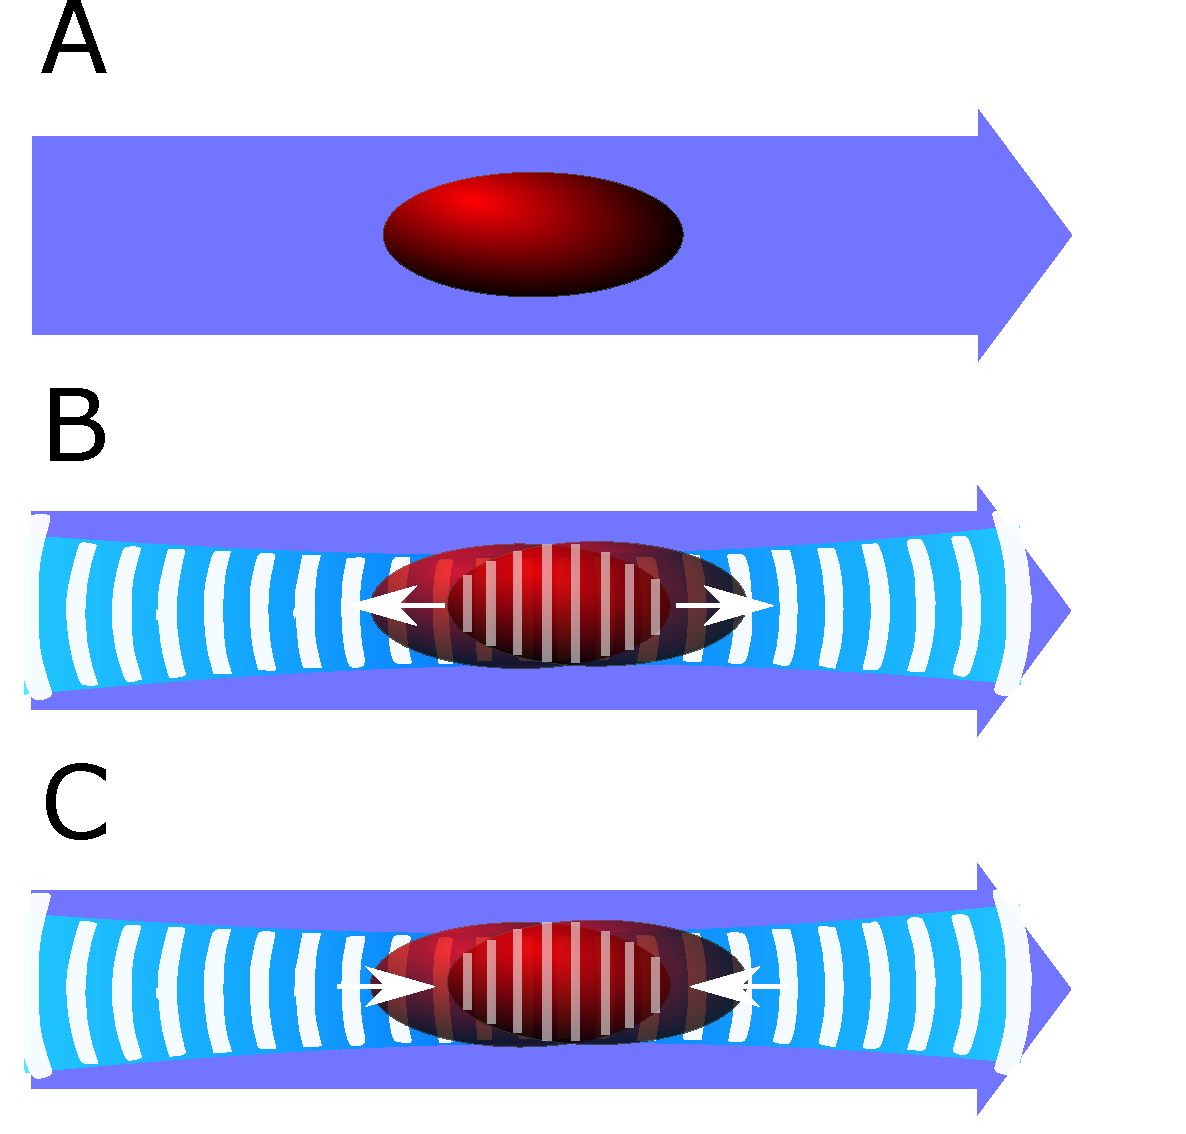
\includegraphics[width=1\columnwidth]{./Figures/KapitzaDirac.pdf}
\caption{In (A) the initial configuration is a ${}^{7}$Li BEC in a harmonic trap illuminated by a laser. (B) The trap is then dropped and the BEC is pulsed with a standing beam which scatters a fraction of the atoms into $\pm 2\hbar n_r k$ states.  (C) After a delay of $1$ ms, a second standing pulse will scatter another group out of the ground group which interfere with the first scattered group.} 
\label{fig:kapitz}
\end{figure}
%*********************************************************

The dipole potential created by a standing wave pulse is given by
\begin{equation}
\mathrm{U(\mathbf{x},t)=\frac{\hbar \Omega_R^2}{\Delta}f^2(t)\sin{(n_rk\mathbf{x})}}
\end{equation}
Where $\Omega_R$ is the Rabi frequency and $\Delta$ is the detuning away from the atomic transition frequency.  Here we have assumed $\Delta^2 \gg \Gamma/4$, where $\Gamma$ is the spontaneous decay rate. The function $f$ can be any function, but here we assume it is a simple step function resulting in a square wave pulse.
In the Raman-Nath approximation, the wave function immediately following a Kapitza-Dirac pulse is \cite{meystre,ketterle}
\begin{equation}
\left|\psi\right>=\left|\psi_0\right>e^{\frac{-i}{\hbar}\int dt'\,U(x,t')}=\left|\psi_0\right>e^{\frac{-i}{2\Delta}\Omega_R^2\tau}e^{\frac{i}{2\Delta}\Omega_R^2\tau\cos{(2n_rkx)}}
\end{equation}
Here we have defined $\tau=\int dt' f^2(t')$ which for a square wave pulse is simply the interaction time $\tau=t_{\mathrm{int}}$.  Note that for Kapitza-Dirac standing wave pulses we are assuming short interaction times relative to the recoil frequency (i.e.\, $t\ll 1/\omega_{\mathrm{rec}}$).  During the pulse we assume the atomic motion is negligible.   Making use of the identity 
\begin{equation}
e^{iA\cos{(B)}}=\sum\limits_{m=-\infty}^{\infty}i^mJ_m(A)e^{imB}
\end{equation}
we rewrite the wave function in terms of Bessel functions of the first kind
\begin{eqnarray}
\left|\psi\right>&=&\left|\psi_0\right>e^{\frac{-i\Omega_R^2\tau}{2\Delta}}\sum\limits_{m=-\infty}^{\infty}i^mJ_m\left(\frac{\Omega_R^2\tau}{2\Delta}\right)e^{i2mn_rkx} \nonumber \\
&=&e^{\frac{-i\Omega_R^2\tau}{2\Delta}}\sum\limits_{m=-\infty}^{\infty}i^mJ_m\left(\frac{\Omega_R^2\tau}{2\Delta}\right)\left|2mn_r\hbar k\right>
\end{eqnarray}
The Hamiltonian after the first pulse has acted is given by
\begin{eqnarray}
\hat{H}&=&\mathrm{\frac{\left(\hat{P}+\mathbf{d}\times\mathbf{B}\right)^2}{2m}-\frac{1}{2}\alpha E^2}\nonumber \\
&=&\mathrm{\frac{\hat{P}^2+2\mathbf{d}\times\mathbf{B}\hat{P}+\left(\mathbf{d}\times\mathbf{B}\right)^2}{2m}-\frac{1}{2}\alpha E^2}\nonumber \\
\end{eqnarray}

This is true since the R\"{o}ntgen term $\mathbf{d}\times\mathbf{B}$ is constant in this setup.  Since plane waves are eigenstates of the Hamiltonian, the eigenvalue of the term $\mathrm{\hat{P}}$ is
\begin{equation}
\mathrm{\hat{P} e^{\pm i2n_rkx}=\pm2n_r\hbar k e^{\pm i2n_rkx}}
\end{equation}
and therefore
\begin{equation}
\mathrm{\hat{H} e^{\pm i2n_rkx}=\left[\frac{\left(\pm 2n_r\hbar k+\mathbf{d}\times\mathbf{B}\right)^2}{2m}-\frac{1}{2}\alpha E^2\right]e^{\pm i2n_rkx}}
\end{equation}
We will drop the phase factor appearing in front of the summation in what follows. From here we can determine the state of the wave function $\psi$ at any time $t$ after the pulse.  In the position space representation this is found to be 
\begin{eqnarray}
&&\mathrm{\psi(x,t+\tau)=e^{\frac{-i\hat{H}t}{\hbar}}\psi(0)} \nonumber \\
&&=\mathrm{J_0\left(\frac{\Omega_R^2\tau}{2\Delta}\right)e^{\frac{-i}{\hbar}\left[\frac{\left(\mathbf{d}\times\mathbf{B}\right)^2}{2m}-\frac{1}{2}\alpha E^2\right]t}\left|0n_r\hbar k\right>} \nonumber \\
&+&\mathrm{iJ_1\left(\frac{\Omega_R^2\tau}{2\Delta}\right)\left(e^{i2n_rkx-\frac{it}{\hbar}\left[\frac{\left( 2n_r\hbar k+\mathbf{d}\times\mathbf{B}\right)^2}{2m}-\frac{1}{2}\alpha E^2\right]}\right)\left|2n_r\hbar k\right>} \nonumber \\
&+&\mathrm{iJ_1\left(\frac{\Omega_R^2\tau}{2\Delta}\right)\left(e^{-i2n_rkx-\frac{it}{\hbar}\left[\frac{\left(-2n_r\hbar k+\mathbf{d}\times\mathbf{B}\right)^2}{2m}-\frac{1}{2}\alpha E^2\right]}\right)\left|-2n_r\hbar k\right>} \nonumber \\
&&=\mathrm{e^{\frac{-it}{\hbar}\left(\frac{\left(\mathbf{d}\times\mathbf{B}\right)^2}{2m}-\frac{1}{2}\alpha E^2\right)}\bigg(J_0\left(\frac{\Omega_R^2\tau}{2\Delta}\right)\left|0n_r\hbar k\right>}\nonumber \\
&&+\mathrm{iJ_1\left(\frac{\Omega_R^2\tau}{2\Delta}\right)e^{i\left(2n_rkx-\frac{4\hbar^2n_r^2k^2t}{2m\hbar}-2n_rk\frac{\mathbf{d}\times\mathbf{B}}{m}t\right)}\left|2n_r\hbar k\right>}\nonumber \\
&&+\mathrm{iJ_1\left(\frac{\Omega_R^2\tau}{2\Delta}\right)e^{i\left(-2n_rkx-\frac{4\hbar^2n_r^2k^2t}{2m\hbar}+2n_rk\frac{\mathbf{d}\times\mathbf{B}}{m}t\right)}\left|-2n_r\hbar k\right>\bigg)}
\end{eqnarray}
Here we have made use of the identity $J_{-m}(\theta)=(-1)^mJ_{m}(\theta)$.  


We next apply another standing wave pulse to this wave function. We are interested in finding the probability of finding the atoms in the ground state $\left|0n_r\hbar k\right>$ after this second pulse, so we are only interested in the $\left|0n_r\hbar k\right>$ terms.
\begin{eqnarray}
&&\mathrm{\psi(x,t+2\tau)=\mathrm{e^{\frac{-it}{\hbar}\left(\frac{\left(\mathbf{d}\times\mathbf{B}\right)^2}{2m}-\frac{1}{2}\alpha E^2\right)}\bigg(J_0^2\left(\frac{\Omega_R^2\tau}{2\Delta}\right)\left|0n_r\hbar k\right>}}\nonumber \\
&&-\mathrm{J_1^2\left(\frac{\Omega_R^2\tau}{2\Delta}\right)e^{i\left(2n_rkx-\frac{4\hbar^2n_r^2k^2t}{2m\hbar}-2n_rk\frac{\mathbf{d}\times\mathbf{B}}{m}t\right)}\left|0n_r\hbar k\right>}\nonumber \\
&&-\mathrm{J_1^2\left(\frac{\Omega_R^2\tau}{2\Delta}\right)e^{i\left(-2n_rkx-\frac{4\hbar^2n_r^2k^2t}{2m\hbar}+2n_rk\frac{\mathbf{d}\times\mathbf{B}}{m}t\right)}\left|0n_r\hbar k\right>\bigg)}
\end{eqnarray}

The probability $p_0$ of finding the atoms in the ground state $\left|0n_r\hbar k\right>$ is

\begin{eqnarray}
\mathrm{p_0=|\left<\psi(x,t+2\tau)|0n_r\hbar k\right>|^2=J_0^4\left(\frac{\Omega_R^2\tau}{2\Delta}\right)}\nonumber \\
\mathrm{-4J_0^2\left(\frac{\Omega_R^2\tau}{2\Delta}\right)J_1^2\left(\frac{\Omega_R^2\tau}{2\Delta}\right)\cos{\left(\frac{4\hbar^2n_r^2k^2t}{2m\hbar}\right)}}\nonumber \\
\mathrm{\times cos{\left(2n_rkx-2\frac{\mathbf{d}\times\mathbf{B}}{m}n_rkt\right)}} \nonumber \\
\mathrm{+4J_1^4\left(\frac{\Omega_R^2\tau}{2\Delta}\right)\cos^2{\left(2n_rkx-2\frac{\mathbf{d}\times\mathbf{B}}{m}n_rkt\right)}}
\label{prob1}
\end{eqnarray}
The third term can be dropped as $J_0^2J_1^2\gg J_1^4$.  

Thus far we have neglected the impact that the doppler shifted dipole term would have on our ability to see the HMW phase.  Without the doppler shift, the dipole term $\frac{1}{2}\alpha E^2$ does not affect the probability since it contributes equally to all momentum states.  The doppler shift presents itself through the detuning 
\begin{equation}
\mathrm{\Delta_{\pm}=\Delta\left(1\pm \frac{\omega_{L}}{\Delta}\frac{v}{c}\right)}
\end{equation}
The doppler shifted dipole term is
\begin{equation}
\mathrm{\frac{1}{2}\alpha\left(1\mp \frac{\omega_{L}}{\Delta}\frac{v}{c}\right)E^2}
\end{equation}
If we include this term, the probability amplitude becomes
\begin{eqnarray}
&&\mathrm{p_0=|\left<\psi(x,t+2\tau)|0n_r\hbar k\right>|^2=J_0^4}\nonumber \\
&&\mathrm{-4J_0^2J_1^2\cos{\left(\frac{4\hbar^2n_r^2k^2t}{2m\hbar}\right)}\cos{\left(2n_rkx-2\frac{\mathbf{d}\times\mathbf{B}}{m}n_rkt+\frac{1}{2}\alpha E^2\frac{\omega_L}{\hbar \Delta}\frac{v}{c}t\right)}} \nonumber \\
&&\mathrm{+4J_1^4\cos^2{\left(2n_rkx-2\frac{\mathbf{d}\times\mathbf{B}}{m}n_rkt+\frac{1}{2}\alpha E^2\frac{\omega_L}{\hbar \Delta}\frac{v}{c}t\right)}} \nonumber \\
&&=J_0^4-\mathrm{-4J_0^2J_1^2\cos{\left(\frac{4\hbar^2n_r^2k^2t}{2m\hbar}\right)}\cos{\left(2n_rkx-2\alpha E^2\frac{n_rkt}{mc}\left(1-\frac{\omega_L}{2\Delta}\right)\right)}} \nonumber \\
\label{prob2}
\end{eqnarray}

Where in the last line we have dropped the higher order term. Comparing  Eq.\ (\ref{prob1}) with  Eq.\ (\ref{prob2}) we see that the dipole effect must be dealt with by running the traveling wave laser in both directions in order to isolate the contribution from the HMW phase.
\vspace{5mm}
 
The HMW phase is incredibly small and requires a large laser intensity to become visible.  We can get a sense of the required magnitude of the HMW to obtain an observable effect by considering the time-frequency uncertainty relation $\Delta \nu \Delta t>1$.  This uncertainty relation tells us that during a 1ms sampling time, we require a frequency shift of $\Delta \nu>$ 1kHz. Setting this equal to the HMW frequency $2\frac{\mathbf{d}\times\mathbf{B}}{m}n_rkt$ we find that $\alpha I>2.3\times 10^{-25}$. Here $I$ is the intensity and $\alpha$ is the polarizability. If we use $\alpha=4\times10^{-36}\,\mathrm{F\cdot m^2}$ as we did in the previous section, then we require a laser intensity of $\mathrm{I=6 \times 10^{6}\,W/cm^2}$. 

Spontaneous emission is a major concern as it affects the visibility of the interference fringes required to observe the HMW effect.  If the separation distance $d$ between the out-coupled sample of atoms in the state $\ket{2\hbar n_r k}$ and the ground atoms $\ket{0\hbar n_r k}$ is larger than the wavelength of the probe laser interacting with the sample, then any spontaneous emission would destroy the coherence of the experiment.  The follows from the fact that under such circumstances, a spontaneous event would allow an observer to positively identify the sample from which the photon was emitted.  This would then break the superposition state of the two samples, thus eliminating the ability to interfere the two states.  
This however is not the case here.  Let us take the dimensions of the condensate to be 300 $\mu$m $\times$ 20 $\mu$m \cite{BEC}. The recoil velocity of Lithium is approximately $\mathbf{v}_{\mathrm{rec}}=9$ cm/s.  Therefore, during the 1 ms that the two samples are separating, the total separation distance is $d=1.8\times 10^{-4}$ m. Therefore the majority of the condensate overlaps throughout the process. Pritchard's group \cite{decoherence} has measured the effects of spontaneous emission on decoherence and has found that for such small separation distances the fringe contrast will not be overly diminished. 

 In free space, such a intensity output would be difficult to achieve, but by placing the atom in a ring cavity (Figure \ref{fig:ringcavity}) we can enhance the intensity by a factor of $2\mathcal{F}/\pi$ \cite{spectroscopy}, where $\mathcal{F}$ is the finesse of the cavity system.  The cavity finesse required will of course depend on the intensity of the pump laser.
A caveat of placing the atom in a cavity system is that a back action of the atom on the intra-cavity field can alter the cavity modes. Collective atom recoil lasing (CARL) instabilities can arise in such a system \cite{courteille}.  CARL labels any type of behavior in a atom-cavity system in which feedback from the atom on the cavity modes cause atomic density modulation and/or growth of optical fields.  As an example of a potential pitfall to placing the atom inside a cavity is the possibility that the atom will radiate into the oppositely traveling mode of the ring cavity and hence setup a lattice.  Such an effect would obviously be undesirable as the dipole force generated by an optical lattice would add an extra layer of complication to disentangling the HMW phase from other effects.  For a single atom massively detuned from the cavity mode, it turns out that even for such high intensities such as those required to see the HMW phase, the CARL threshold is not reached \cite{hemmerich} and the back action effects may safely be ignored.  
%***************************figure**********************
\begin{figure}[htp]
\includegraphics[width=1\columnwidth]{./Figures/RingCavity.pdf}
\caption{A schematic for the high finesse ring cavity setup used to enhance the intensity of the traveling wave. The cavity mode must be massively detuned from the atomic transition in order to suppress spontaneous emission $\gamma$. } 
\label{fig:ringcavity}
\end{figure}
%*********************************************************

Using a Kaptiza-Dirac pulse of wavelength $\lambda=671\,\mathrm{nm}$ the value of the recoil frequency term is $n_r\hbar kx =3.4\times 10^3$, while $\frac{4\hbar^2n_r^2k^2t}{2m\hbar}$ is approximately twice the size of the recoil term. The R\"{o}ntgen term which is responsible for the HMW phase is  $2\frac{\mathbf{d}\times\mathbf{B}}{m}n_rk\,t=9.5\,t$/s.  
In figure \ref{fig:ft2hk} we plot the probability of finding the atom in the ground state (Eq.\ (\ref{prob1})) with and without the HMW phase using these values. The red line shows the probability to find the atoms in the ground state without the HMW phase, while the solid blue lines include the HMW phase. In \ref{fig:ft2hk} we plot the Fourier transform.  
%***************************figure**********************
\begin{figure}[htp]
\includegraphics[width=1\columnwidth]{./Figures/Probability2hknew.pdf}
\caption{A plot of the probability of finding the atoms in the ground state $\mathrm{p_0=|\left<\psi(x,t+2\tau)|0n\hbar k\right>|^2}$. The red line show the probability of finding the atoms in the ground state without the HMW phase, while the blue line include the HMW phase. The intensity of the laser is $I_1=9.7\times 10^6\, \mathrm{W/cm^2}$.} 
\label{fig:prob}
\end{figure}
%*********************************************************
%***************************figure**********************
\begin{figure}[htp]
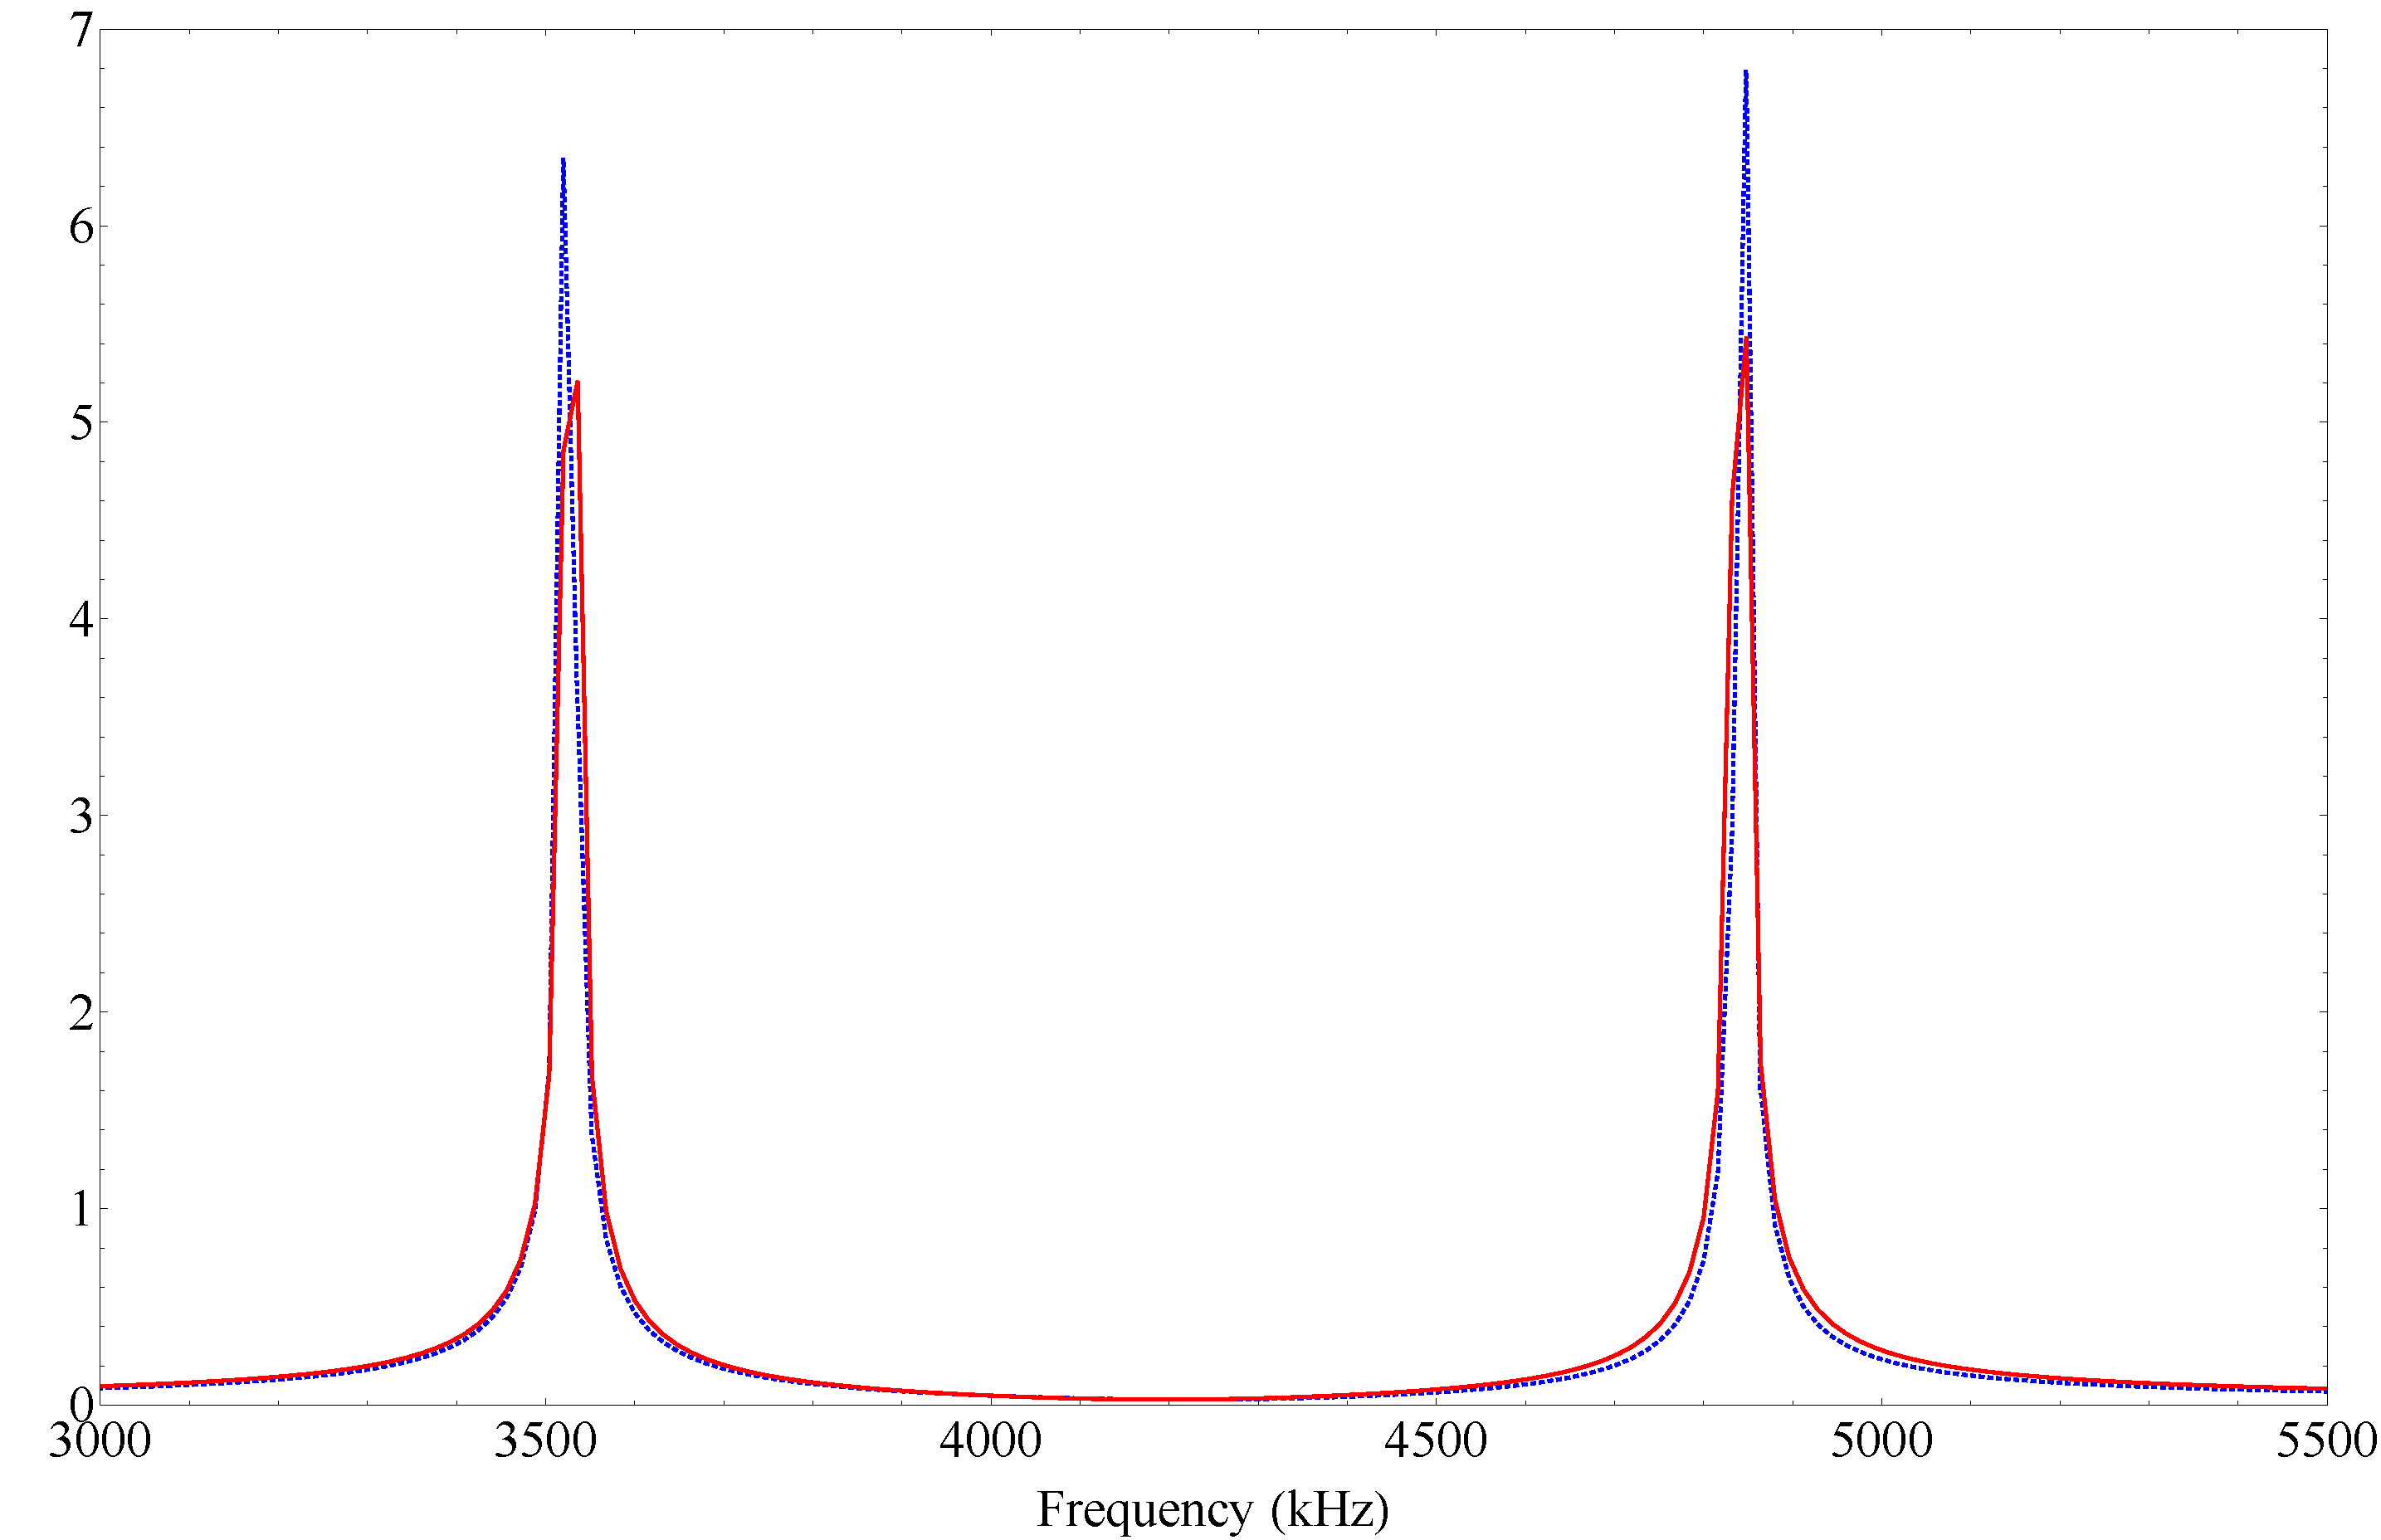
\includegraphics[width=1\columnwidth]{./Figures/FT2hk.pdf}
\caption{The time-discrete fourier transform of Eq.\ (\ref{prob1}) using 1 ms of sampling with a 1 $\mu$s sample rate. The dotted blue line shows the fourier transform without the HMW phase, while the red line include the HMW phase. The effect of the HMW on the Fourier transform is most apparent in the magnitude change, while the frequency shift is difficult to see. It is important to note that we chose parameters in which the difference is just beginning to emerge.} 
\label{fig:ft2hk}
\end{figure}
%*********************************************************


A possible enhancing technique which may also be implemented to increase the size of the R\"{o}ntgen term is to consider large momentum transfer beamsplitters (LMT). Thus far we have only considered recoil momentum kicks of the form $2n_r\hbar k$. However, it is possible to use large momentum transfers on the order of $10 n_r\hbar k-100 n_r\hbar k$ \cite{kasevich}.  Using such an LMT, we would could significantly increase the effects of the HMW phase.  This however also works against us by increasing the separation distance between samples, and hence decreasing the fringe visibility.  A better option is to simply increase the intensity slightly at the cost of a modest decrease in visibility due to spontaneous emission.  In Figures \ref{fig:prob10} and \ref{fig:ft10hk} we plot Eq.\ (\ref{prob1}) and the time-discrete Fourier transform using an intensity of $I_2=9.7\times 10^7\, \mathrm{W/cm^2}$.

%***************************figure**********************
\begin{figure}[htp]
\includegraphics[width=1\columnwidth]{./Figures/Probability10hknew.pdf}
\caption{A plot of the probability of finding the atoms in the ground state $\mathrm{p_0=|\left<\psi(x,t+2\tau)|0n\hbar k\right>|^2}$. The red line show the probability of finding the atoms in the ground state without the HMW phase, while the blue line include the HMW phase. Here the difference between the two is more apparent. The intensity of the laser is set to $I_1=9.7\times 10^7\, \mathrm{W/cm^2}$.} 
\label{fig:prob10}
\end{figure}
%*********************************************************
%***************************figure**********************
\begin{figure}[htp]
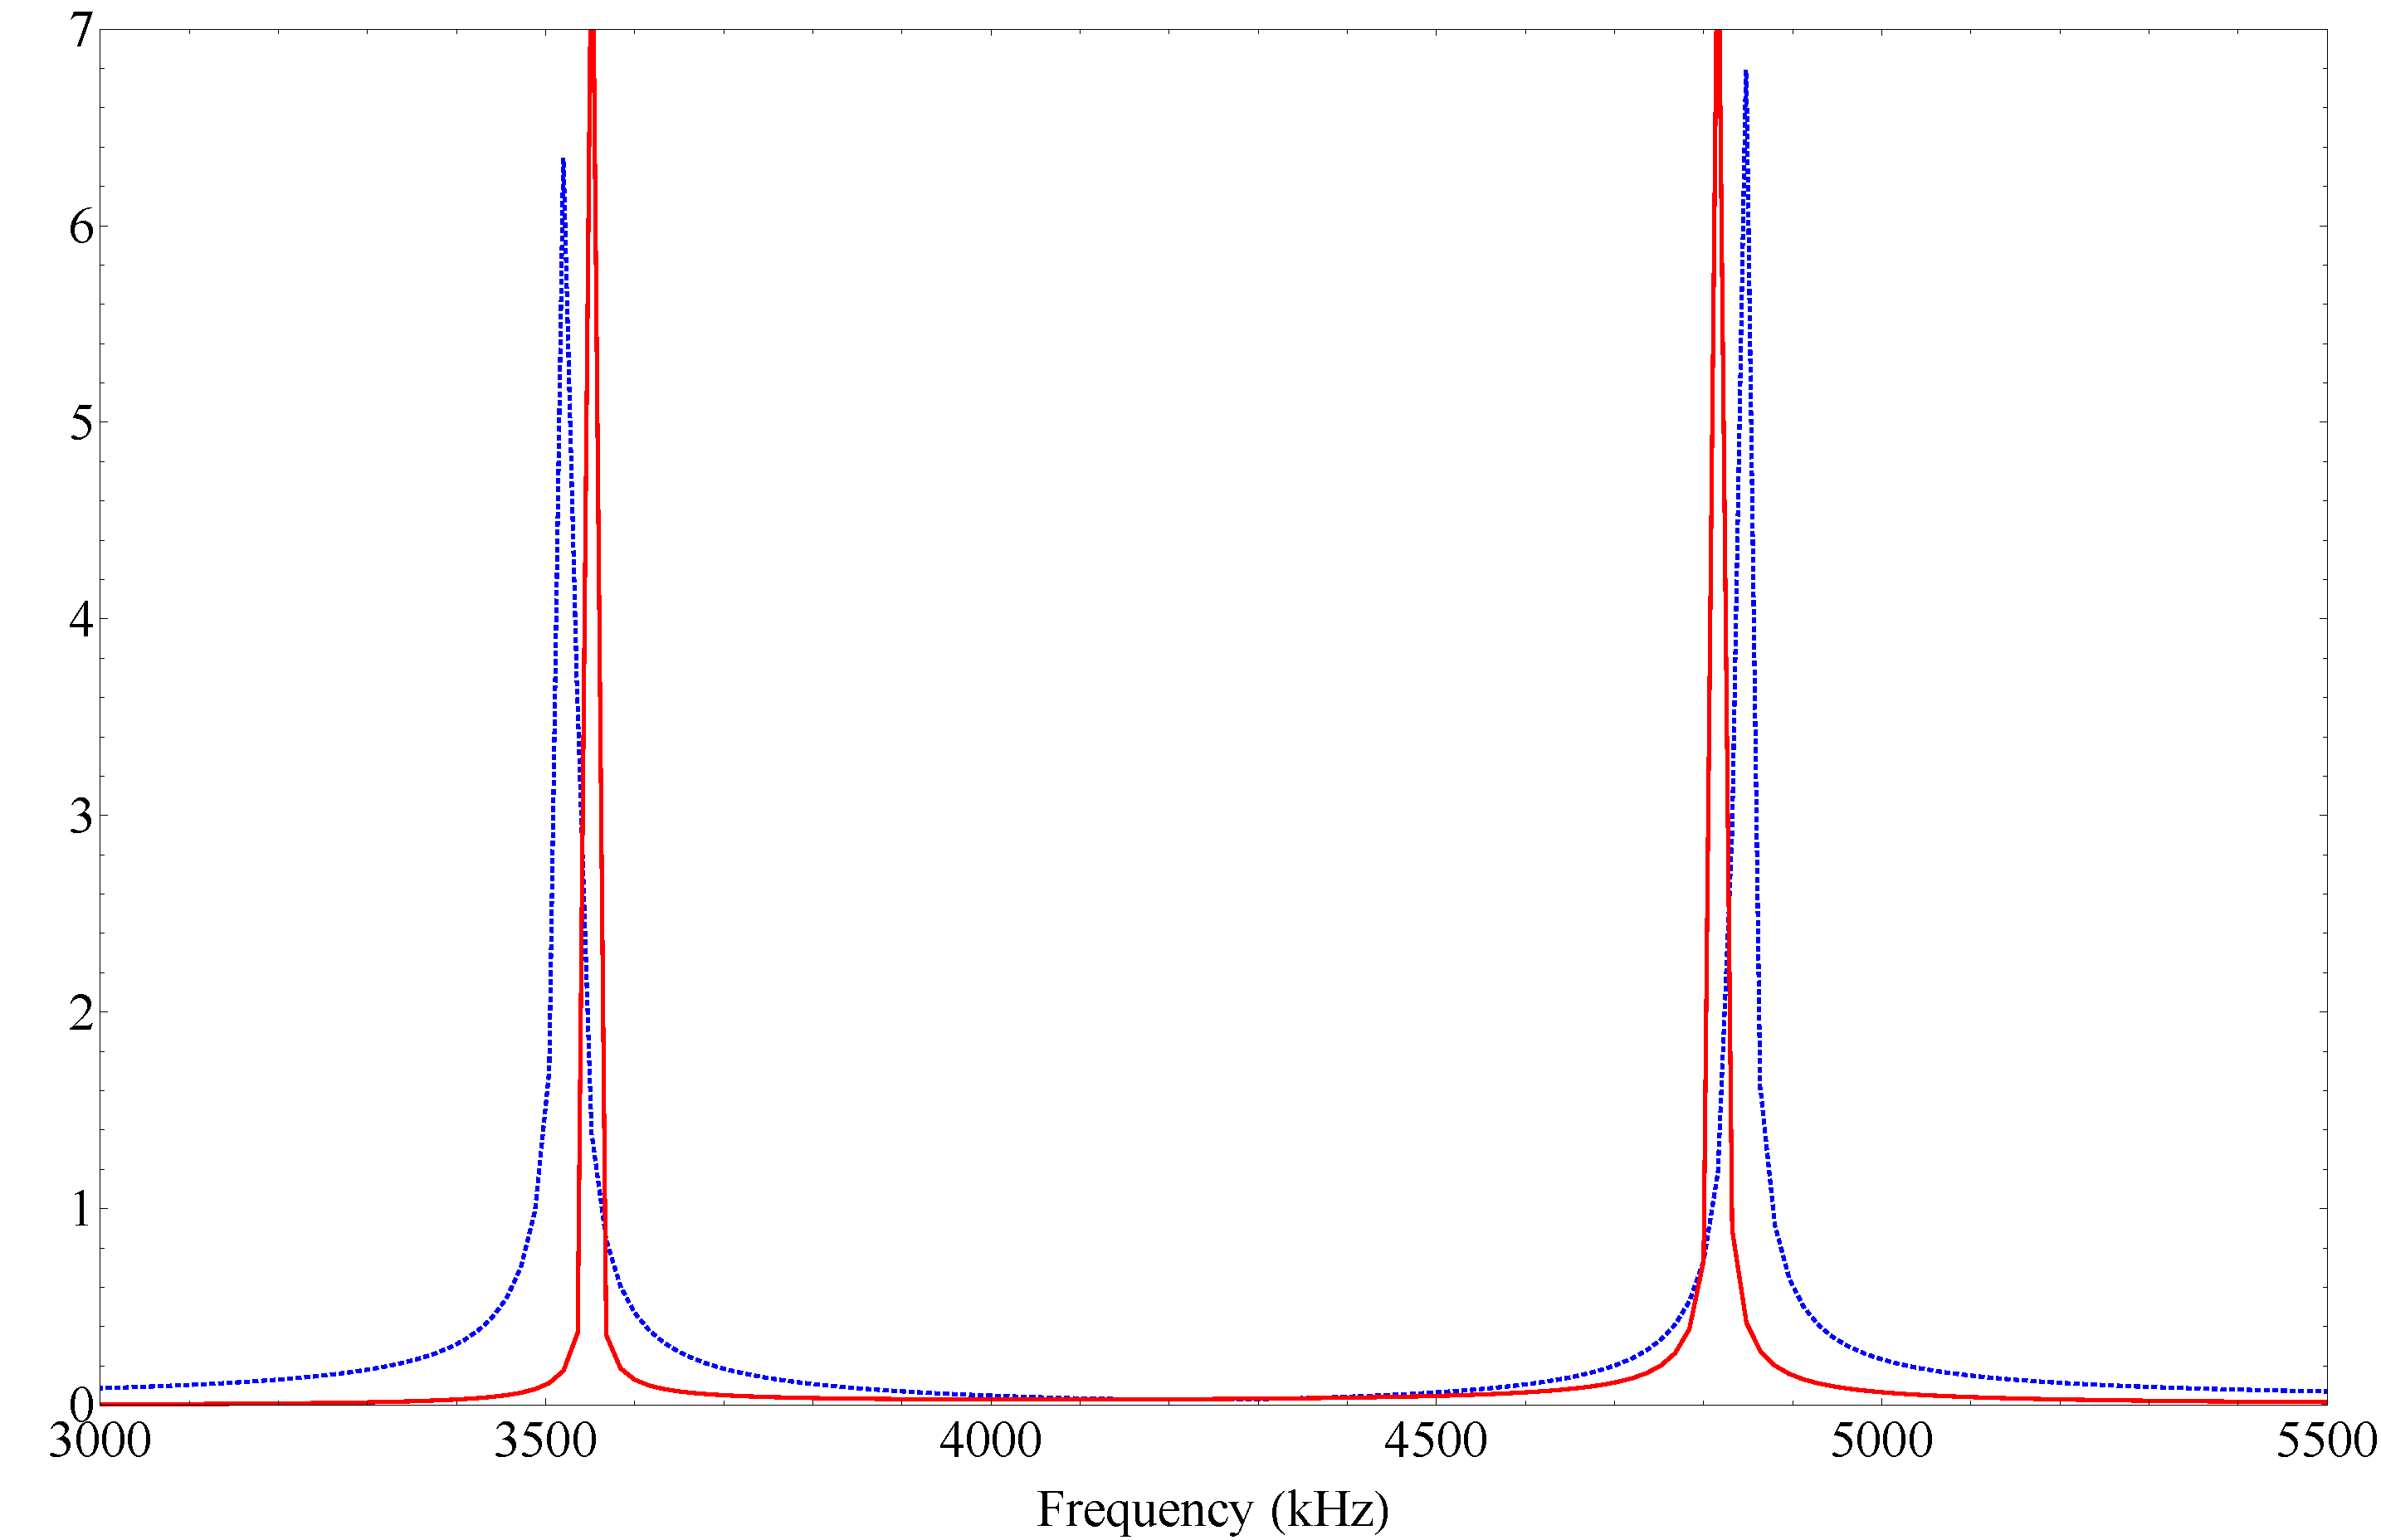
\includegraphics[width=1\columnwidth]{./Figures/FT10hk.pdf}
\caption{The time-discrete fourier transform of Eq.\ (\ref{prob1}) using an increased intensity $I_1=9.7\times 10^7\, \mathrm{W/cm^2}$.  The separation between the peaks is much more striking here.} 
\label{fig:ft10hk}
\end{figure}

%*********************************************************




%==============================
\newpage
\section{Laguerre Beams}
The setup we consider is a trapped BEC in an optical ring trap as outlined in \cite{phillips, boshier}.  The BEC is then irradiated with a single Laguerre-Gaussian (LG) beam. Note that this is different from typical setups \cite{campbell} in which the Laguerre-Gauss beam is accompanied by a counter-propagating Gaussian beam.  The interaction of the two beams creates a standing wave profile, producing a dipole force on the BEC which is responsible for the transfer of angular momentum. What we wish to show is that the HMW phase can be observed from a setup in which only a single LG beam is present. Consider an LG mode $L_0^l$, linearly polarized in the transverse x-direction as shown in figure \ref{fig:setup}.  The magnitude of the Laguerre-Gauss mode $u_0^l$ at $z=0$ can be written in cylindrical coordinates as \cite{Willke}
\begin{equation} 
\mathrm{u_0^l(\bold{r,\phi})=A_0 \sqrt{\frac{2}{\pi w_0^2}}\sqrt{\frac{1}{l!}}\exp{\frac{-2r^2}{w^2}}\left(\frac{\sqrt{2}r}{w}\right)^{l}\exp{il\phi}}
\label{LGmode}
\end{equation}
%***************************figure**********************
\begin{figure}[htp]
\includegraphics[width=1\columnwidth]{./Figures/azimuthal.pdf}
\caption{A Laguerre-Gauss field with linear polarization acts on an atomic circuit trap. The wavefronts of the beam have an azimuthal component giving the Poynting vector a non-zero angular term.  This acts on the atom circuit to generate an azimuthal flow.} 
\label{fig:setup}
\end{figure}
%*********************************************************
where $A_0$ is the amplitude, and $w_0$ is the beam waist. The vector potential $\mathrm{A(\bold{r,\phi,z})}$ associated with such a mode can be written as
\begin{equation} 
\mathrm{A(\bold{r,\phi,z})}=\mathrm{u_0^l(\bold{r,\phi})\exp{i(\bold{kz}-\omega t)}\hat{\bold{x}}}
\label{vpotential}
\end{equation}
The electric and magnetic fields may then be obtained via
\begin{eqnarray}
&&\mathrm{E(\bold{r,\phi,z})= i\omega \left(A(\bold{r,\phi,z})+\frac{\nabla\left(\nabla\cdot A(\bold{r,\phi,z})\right)}{k^2}\right)} \nonumber \\
&&\mathrm{B(\bold{r,\phi,z})=\nabla\times A(\bold{r,\phi,z})}
\end{eqnarray}
We apply the paraxial approximation in which we neglect terms which have derivatives in the longitudinal direction (z-direction) along with higher derivatives of the transverse components
\begin{eqnarray}
&&\mathrm{E(\bold{r,\phi,z})= i\omega u(\bold{r,\phi})\exp{i(\bold{kz}-\omega t)}\hat{\bold{x}} -c \frac{\partial u(\bold{r,\phi})}{\partial x}\exp{i(\bold{kz}-\omega t)}\hat{\bold{z}}} \nonumber \\
&&\mathrm{B(\bold{r,\phi,z})=ik u(\bold{r,\phi})\exp{i(\bold{kz}-\omega t)}\hat{\bold{y}}-\frac{\partial u(\bold{r,\phi})}{\partial x}\exp{i(\bold{kz}-\omega t)}\hat{\bold{z}}} \nonumber \\
\end{eqnarray}
We first wish to find the azimuthal component of $\mathcal{\alpha E\times B}$.  
\begin{equation}
\mathrm{\left(\alpha E\times B\right)_{\phi}=\frac{4A_0^2 \alpha ck 2^l}{w_0^{2l+2} \pi l!}r^{2l}\exp{\frac{-2r^2}{w^2}}\left[\frac{2}{w_0^2}-lr^{-2}\right]}
\end{equation}
This term is the only component responsible for giving us an HMW phase around a circuit.  However, since we also wish to write the LG mode in terms of the output power of the laser $P$, we also want the z-component of $E\times B$ in order to find the intensity of the laser.  
\begin{equation}
\mathrm{\left(\alpha E\times B\right)_{z}=\frac{c^2 k^2 A_0^2 2^l}{w_0^{2l+2} \pi l!}r^{2l}\exp{\frac{-2r^2}{w^2}}}
\end{equation}
The intensity of a beam is given by $\mathrm{I=\frac{1}{2}\epsilon_0 c^2 \left(\alpha E\times B\right)_{z}}$ which can be rewritten as $\mathrm{I=\frac{1}{2}\epsilon_0 c^2 k^2 A_0^2 |u_0^l|^2}$ in terms of the LG modes.  Integrating this over the area gives the power $\mathrm{P=\frac{1}{2}\epsilon_0 c^2 k^2 A_0^2}$ which is simple as the LG modes are normalized.  This yields $\mathrm{A_0=\sqrt{\frac{2P}{\epsilon_0 c^2 k^2}}}$
From here we can work out the HWM phase by making use of the curl theorem $\mathcal{\int\!\left(\nabla \times \bold{A}\right)\cdot\! d\bold{a}=\oint \!\bold{A}\cdot \!d\bold{l}}$ 
\label{HMW}
\begin{equation}
\mathrm{\exp{iS/\hbar}=i\frac{16P \alpha ck 2^l}{\hbar w_0^{2l+2} \epsilon_0 ck l!}\int_0^a\!\exp{\frac{-2r^2}{w^2}}\left[ \frac{2}{w_0^2}r^{2l+1}-lr^{2l-1}\right]\!dr}
\end{equation}
where $\mathrm{a}$ is the radius of the atom circuit produced by the trap.  This integral can be solved analytically 
\begin{equation}
\mathrm{\int_0^a\!\exp{\frac{-2r^2}{w^2}}\left[ \frac{2}{w_0^2}r^{2l+1}-lr^{2l-1}\right]\!dr = -\frac{1}{2}\exp{\frac{-2a^2}{w^2}}a^{2l}}
\end{equation}
The maximum value for which occurs at a radius of $\mathrm{a=w_0/sqrt{2}}$.  Plugging this into Eq.\ (\ref{HMW}) gives a maximum phase of
\begin{equation}
\mathrm{\exp{iS/\hbar}=exp{\left(-i\frac{8P \alpha 2^l}{\hbar e^1 w_0^{2} \epsilon_0 ck l!}\right)}}
\end{equation}
Recently Willke's \cite{Willke} group was able to generate high order ($u^3_3$) Laguerre-Gauss beams with high laser power (83 Watt). Using $\alpha=9.6\times10^{-35}{\mathrm{cm}}^2\mathrm{V}$ along with the parameters used by Willke's group we find the HMW phase shift to be approximately $-4\times10^5$ radians. 
We begin with the Hamiltonian for a BEC in an elliptical trap interacting
with a Laguerre-Gauss beam.
\[
i\hbar\partial_{t}\psi=H\psi=\left[-\frac{\hbar^{2}}{2m}\left(\frac{1}{R}\frac{\partial}{\partial\theta}+\frac{i}{\hbar}\vec{d}\times\vec{B}\right)^{2}-V_{0}\cos\theta\right]\psi
\]
The potential amplitude $V_{0}$ can be adjusted as needed. The Poynting
term $\vec{d}\times\vec{B}$ is given by:
\[
\vec{d}\times\vec{B}=\frac{-4\alpha P}{c^{2}\epsilon_{0}k\pi w_{0}^{4}}re^{-2r^{2}/w_{0}^{2}}\equiv C_{1}re^{-2r^{2}/w_{0}^{2}}
\]
where$w_{0}$is the gaussian beam width, $r$ is the radius, $P$
is the power of the beam, and$\alpha$ is the atomic polarizibility.
We are now ready to expand out the Hamiltonian and see what we get.
Let $\psi=e^{in\theta}/\sqrt{2\pi R}$

\[
H\psi=\left[-\frac{\hbar^{2}}{2m}\left(\frac{1}{R}\frac{\partial}{\partial\theta}+\frac{i}{\hbar}\vec{d}\times\vec{B}\right)^{2}-V_{0}\cos\theta\right]\psi
\]


\[
=\left[-\frac{\hbar^{2}}{2m}\left(-\left(\frac{n}{R}\right)^{2}-2\frac{1}{\hbar}\vec{d}\times\vec{B}\left(\frac{n}{R}\right)-\left(\frac{\vec{d}\times\vec{B}}{\hbar}\right)^{2}\right)-V_{0}\cos\theta\right]\frac{e^{in\theta}}{\sqrt{2\pi R}}
\]


\[
=\left[\frac{\hbar^{2}}{2m}\left(\frac{n}{R}+\frac{\vec{d}\times\vec{B}}{\hbar}\right)^{2}-V_{0}\cos\theta\right]\frac{e^{in\theta}}{\sqrt{2\pi R}}
\]
Now what this tells us is that in order to go from the $n=0$ parabola
to the $n=1$ we require $\frac{\vec{d}\times\vec{B}}{\hbar}=\frac{1}{r}$.
This tells us the laser power we need to input in order to get any
rotation. Note this has nothing to do with the speed at which we are
sweeping, we simply want to know how much power we will need to see
any rotation. Our requirment for the Poynting vector to be strong
enough to generate a vortex is given by

\[
\frac{4\alpha P}{\hbar c^{2}\epsilon_{0}k\pi w_{0}^{4}}re^{-2r^{2}/w_{0}^{2}}=\frac{1}{r}
\]
where $P$ is the power, and $w_{0}$ is the beam waist length. We
also make use Duncan's equations for the dynamic polarizibility $\alpha$

\[
\alpha\left(\omega_{L}\right)=\frac{1}{\hbar}\left(\frac{\mu_{A}^{2}}{\Delta+2\pi\times267\times10^{6}}+\frac{\mu_{B}^{2}}{\Delta}\right)
\]
where $\mu_{A}\approx\mu_{B}\approx1.45\times10^{-29}$Cm, and $\Delta$
is the detuning. The spontaneous emission scattering rate $\Gamma_{sc}$
is given by

\[
\Gamma_{sc}=\frac{3\pi c^{2}}{2\hbar\omega_{0}^{3}}\left(\frac{\Gamma}{\Delta}\right)^{2}I=\frac{6c^{2}\Gamma^{2}P}{\sqrt{2}\hbar\omega_{0}^{3}w_{0}^{3}k\Delta^{2}}
\]
Where $\omega_{0}=2\pi\times3.84\times10^{14}s^{-1}$ is the D2-line
transition frequency, $\Gamma=3.61\times10^{7}s^{-1}$ is the natural
line width. Here we used the intensity $I$ at $r=w_{0}/\sqrt{2}$
given by

\[
I=\frac{1}{2\mu_{0}}E\times B=\frac{4P}{\pi w_{0}^{4}k}re^{-2r^{2}/w_{0}^{2}}=\frac{4P}{\sqrt{2}\pi w_{0}^{3}k}
\]
Rearranging the scattering rate equation and solving for the power
$P$ yields

\[
P=\frac{\sqrt{2}\hbar\omega_{0}^{3}w_{0}^{3}k\Delta^{2}\Gamma_{sc}}{6c^{2}\Gamma^{2}}
\]
We can then plug this into the equation
\[
\frac{4\alpha P}{\hbar c^{2}\epsilon_{0}k\pi w_{0}^{4}}re^{-2r^{2}/w_{0}^{2}}=\frac{1}{r}
\]
\[
\Rightarrow\frac{\sqrt{2}\omega_{0}^{3}w_{0}\alpha\Delta^{2}\Gamma_{sc}}{3c^{4}\epsilon_{0}\pi\Gamma^{2}}=1
\]
This now gives us a relationship between the different parameters
involved. Our job is to find a sweet spot in which the scattering
rate is managable. We now substitute in the formula for the dynamic
polarizibility $\alpha$ in the limit where detuning dominates. In
this limit we have

\[
\alpha\left(\omega_{L}\right)\approx\frac{2}{\hbar}\frac{\mu_{B}^{2}}{\Delta}
\]
and obtain
\[
\frac{2\sqrt{2}\omega_{0}^{3}w_{0}\mu_{B}^{2}\Delta\Gamma_{sc}}{3\hbar c^{4}\epsilon_{0}\pi\Gamma^{2}}=1
\]
Solving this for the scaterring rate $\Gamma_{sc}$

\[
\Gamma_{sc}=\frac{3\hbar c^{4}\epsilon_{0}\pi\Gamma^{2}}{2\sqrt{2}\omega_{0}^{3}w_{0}\mu_{B}^{2}\Delta}
\]
Let's now assume we are using a $CO_{2}$ with a wavelength of $10\times10^{-6}$m,
and frequency $3\times10^{13}$. This would give us a massive detuning
of $\Delta\thickapprox\omega_{0}$. Plugging in the values of the
other parameters which are found above, gives us

\[
\Gamma_{sc}=\frac{4.4}{w_{0}}
\]
We can see that the scattering rate is actually quite small, as long
as we keep the radius of the trap large. Let the radius be $r=5\times10^{-6}$,
then the scattering rate is approximately $10^{6}$. This gives us
a time frame of about $10^{-6}$s. The power $P$ needs to be quite
large as a result

\[
P=\frac{\hbar c^{2}\epsilon_{0}k\pi w_{0}^{2}}{2\alpha}=5.5\times10^{5}
\]
The Landau-Zener formula which states that the probability of making
a diabatic transition is given by

\[
P=e^{-2\pi\Theta}
\]


\[
\Theta=\frac{d^{2}/\hbar}{\frac{d}{dt}\left(E_{1}-E_{0}\right)}
\]
where $d$ is the off diagona\textbackslash{}frac\{4\textbackslash{}alpha
P\}\{\textbackslash{}hbar c\textasciicircum{}\{2\}\textbackslash{}epsilon\_\{0\}k\textbackslash{}pi
w\_\{0\}\textasciicircum{}\{4\}\}re\textasciicircum{}\{-2r\textasciicircum{}\{2\}/w\_\{0\}\textasciicircum{}\{2\}\}l
element in the Hamiltonian. For our system, this term corresponds
to $V_{0}/2$. We can find the energy difference easily enough.

\[
E_{0}=\frac{\hbar^{2}}{2m}\left(\frac{\vec{d}\times\vec{B}}{\hbar}\right)^{2}-V_{0}
\]


\[
E_{1}=-\frac{\hbar^{2}}{2m}\left(-\left(\frac{1}{r}\right)^{2}-2\frac{1}{\hbar}\vec{d}\times\vec{B}\left(\frac{1}{r}\right)-\left(\frac{\vec{d}\times\vec{B}}{\hbar}\right)^{2}\right)-V_{0}
\]
Then we get
\[
\frac{d}{dt}\left(E_{1}-E_{0}\right)=2\frac{\hbar}{mr}\frac{d}{dt}\left(\vec{d}\times\vec{B}\right)
\]
We next need to determine how fast we need to sweep at to go from
one parabola to the other in the allotted time (i.e before spontaneous
emission burns us). Well the time doesn't seem to be a problem so
let's sweep from $\vec{d}\times\vec{B}=0$ to the necessary $\vec{d}\times\vec{B}=\hbar/r$
intensity linearly in 1s. Plugging this into the Landau-Zener equation
we get

\[
\Theta=\frac{V_{0}^{2}/4\hbar}{2\frac{\hbar^{2}}{mr^{2}}}=\frac{V_{0}^{2}mr^{2}}{8\hbar^{3}}
\]
Now if $V_{0}$ is the potential due to gravity
\[
V_{0}=-G\frac{M_{E}m}{r}=-1.0\times10^{-17}N/m
\]
Using this value, even though it's small we'll still get perfectly
adiabatic following.





%==============================
\section{Summary and Conclusions}

yup

%================================================================
